\documentclass{beamer}
\usepackage{caption}
\usepackage{float}
\usepackage{lscape}
\usepackage{graphicx}% http://ctan.org/pkg/graphicx
\usepackage{booktabs}% http://ctan.org/pkg/booktabs
\usepackage{array}
\usepackage[export]{adjustbox}
\usepackage{amsmath}
\usepackage{amsfonts}
\usepackage{amssymb}
\usepackage{tikz}
\usepackage{ upgreek }
\usepackage{subcaption}
\usepackage{tabularx} 
\usepackage{setspace}



\graphicspath{ {images/} }
\usetheme{Madrid}
\definecolor{Gold}{RGB}{218,165,32}
\setbeamertemplate{navigation symbols}{}
\setbeamertemplate{theorems}[numbered]
\setbeamertemplate{theorems}[ams style] 
\renewcommand{\qedsymbol}{$\blacksquare$}

\makeatletter

\setbeamerfont{footline}{size=\fontsize{6}{8.5}\selectfont}

\defbeamertemplate*{footline}{Dan P theme}
{
  \leavevmode%
  \hbox{%
  \begin{beamercolorbox}[wd=.15\paperwidth,ht=2.25ex,dp=1ex,center]{author in head/foot}%
    \usebeamerfont{author in head/foot}\insertshortauthor\expandafter\beamer@ifempty\expandafter{\beamer@shortinstitute}{}{~~(\insertshortinstitute)}
  \end{beamercolorbox}%
  \begin{beamercolorbox}[wd=.63\paperwidth,ht=2.25ex,dp=1ex,center]{title in head/foot}%
    \usebeamerfont{title in head/foot}\insertshorttitle
  \end{beamercolorbox}%
  \begin{beamercolorbox}[wd=.22\paperwidth,ht=2.25ex,dp=1ex,right]{date in head/foot}%
    \usebeamerfont{date in head/foot}\insertshortdate{}\hspace*{1.5em}
\insertframenumber{} / \inserttotalframenumber\hspace*{4ex} 
  \end{beamercolorbox}}%
  \vskip0pt%
}
\makeatother

\title{Cross-Industry Dispersion and the Cross-Section of Expected Returns \\ (Pinchuk 2019)}

% A subtitle is optional and this may be deleted
%\subtitle{Optional Subtitle}

\author{Mykola Pinchuk}

\date{11/05/2019}

\subject{Empirical Asset Pricing}

\AtBeginSubsection[]

\begin{document}

\begin{frame}
  \titlepage
\end{frame}



\begin{frame}{Introduction}
\begin{itemize}
    \item {The economy has permanently evolving structure.}
    \item {Accelerated rate of sectoral reallocation creates unemployment risk for workers in declining industries.}
    \item {Many workers possess significant industry-specific skills.}
    \item {Sectoral shifts create large labor income risk for workers with industry-specific skills.}
    \item {Since employees can not fully hedge labor income risk, it should be relevant for asset pricing.}
    \item {\textbf{Is the rate of sectoral shifts a state variable?}}
\end{itemize}

\end{frame}


\begin{frame}{Key results}
\begin{itemize}
    \item {I use cross-industry dispersion (CID) to measure the rate of sectoral shifts.}
    \item {CID is the cross-sectional mean absolute deviation of the returns of industry portfolios.}
    \item {Stocks with high sensitivity to CID produce low returns.}
    \item {This return spread (68 bps) is not explained by common factors.}
    \item {Unlike CID, within-industry dispersion (WID) is not priced.}
    \item {Consistent with the hypothesis that CID proxies for labor risk from sectoral shifts, CID predicts unemployment.}
\end{itemize}
\end{frame}



\begin{frame}{Literature}{Related asset pricing literature on idiosyncratic risk}
\begin{itemize}
    \item {Theory:}
    \begin{itemize}
        \item {Constantinides and Duffie (1996): Heterogeneous-agent model, where cross-sectional variance of income growth is a state variable.}
    \end{itemize}
    \item {Empirical papers on idiosyncratic risk:}
    \begin{itemize}
        \item {Ang, Hodrick, Xing and Zhang (2006): High sensitivity to VIX is related to low returns.}
        \item {Herskovic, Kelly, Lustig and Van Nieuwerburgh (2016): High sensitivity to common idiosyncratic volatility (CIV) is related to low returns.}
        \item {Verousis and Voukelatos (2018): High sensitivity to cross-sectional dispersion (CSD) is related to low returns.}
    \end{itemize}
\end{itemize}
\end{frame}



\begin{frame}{Literature}{Macroeconomic literature on unemployment and sectoral shifts}
\begin{itemize}
    \item {Lilien (1982): Unemployment is driven by two forces: aggregate shocks and sectoral shifts. Most of employment fluctuations in 1970s were driven by sectoral reallocation shocks.}
    \item {Loungani, Rush and Tave (1990): Sectoral shifts, proxied by the index of stock market dispersion, predict unemployment at the annual frequency.}
    \item {Brainard and Cutler (1993): Sectoral reallocation shocks account for a large fraction of the variation in long-term unemployment.}
\end{itemize}
\end{frame}



\begin{frame}{Relationship to literature}
\begin{itemize}
    \item {Bridges the gap between macro and asset pricing literature.}
    \item {Shows asset pricing implications of unemployment, driven by sectoral shifts.}
    \item {Provides evidence, broadly consistent with the model of Constantinides and Duffie (1996).}
    \item {Provides fundamental economic explanation for the cross-sectional returns predictability by CSD (Verousis and Voukelatos 2018).\\
    This predictability is driven by the cross-industry component of CSD (i.e., CID).}
\end{itemize}
\end{frame}



\begin{frame}{Data}
\begin{itemize}
    \item {CRSP 1926-2018 and Compustat 1963-2018.}
    \item {Fama-French industry portfolios and factors from French`s website.}
    \item {Uncertainty indices from Ludvigson`s website.}
    \item {Unemployment data from Bureau of Labor Statistics.}
\end{itemize}
\end{frame}



\begin{frame}{Cross-Industry Dispersion}
\begin{itemize}
    \item {Cross-Industry Dispersion (CID) is the mean absolute deviation of the returns of FF49 industry industries.}
    \item {I measure CID at the daily frequency: \\
    $$CID_t = \frac{1}{N}\sum^{N}_{i=1}{|R_{it}-R_{MKT,t}|}.$$}
    \item {In every period, I use only the industries with at least 10 firms, so $N \leq 49$.}
    \item {I compute within-industry dispersion (WID) as the mean absolute deviation between stock returns and value-weighted return of its industry:
    $$WID_t = \frac{1}{N}\sum^{N}_{j=1}\frac{1}{M_j}\sum^{M_j}_{i=1}{|R_{it}-R_{jt}|}.$$}
\end{itemize}
\end{frame}



\begin{frame}{Time series of CID}
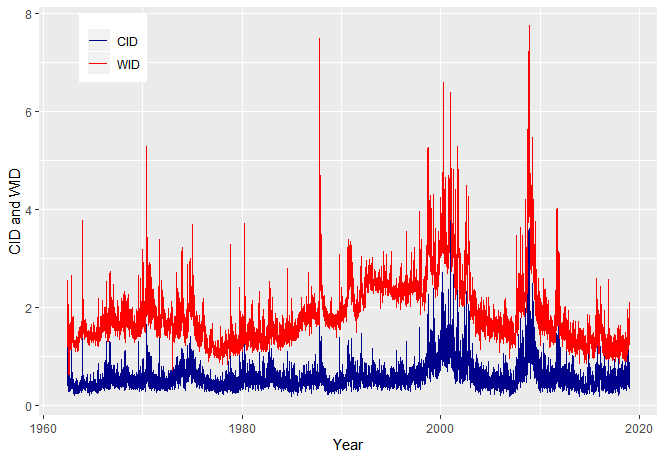
\includegraphics[width=1\textwidth]{paper_b3/Figure1_sl.png}
\end{frame}



\begin{frame}{Cross-Industry Dispersion}
\begin{table}[!htbp] \centering 
  \caption*{\textbf{Table 1: Correlations of changes in CID with changes in other variables}} 
  \label{} 
    \begin{flushleft}
    {\medskip\scriptsize
 The table reports correlations between changes in CID and changes in other variables at the monthly frequency. VIX is implied volatility, available starting from 1990. FU and MU are financial and macroeconomic uncertainty from Sydney Ludvigson website. VOL is the volatility of monthly value-weighted market index over the recent 24 months. CIV is common idiosyncratic volatility (Herskovic et al., 2016). }
    \medskip
    \end{flushleft}
\small
\vspace{-0.1cm}
\begin{tabular}{@{\extracolsep{5pt}} ccccccc} 
\\[-1.8ex]\hline 
\hline \\[-1.8ex] 
 & VIX & FU & MU & VOL & CIV & CID \\ 
\hline \\[-1.8ex] 
VIX & $1$ & $0.40$ & $0.36$ & $0.34$ & $0.50$ & $0.11$ \\ 
FU & $0.40$ & $1$ & $0.44$ & $0.30$ & $0.39$ & $0.18$ \\ 
MU & $0.36$ & $0.44$ & $1$ & $0.11$ & $0.24$ & $0.06$ \\ 
VOL & $0.34$ & $0.30$ & $0.11$ & $1$ & $0.27$ & $0.27$ \\ 
CIV & $0.50$ & $0.39$ & $0.24$ & $0.27$ & $1$ & $0.22$ \\ 
CID & $0.11$ & $0.18$ & $0.06$ & $0.27$ & $0.22$ & $1$ \\ 
\hline \\[-1.8ex] 
\end{tabular} 
\end{table}
\end{frame}




\begin{frame}{Estimation of $\beta_{CID}$}
\begin{itemize}
    \item {I difference and residualize $CID_t$ using the specification from Pastor and Stambaugh (2003):
    $$\Delta(CID_t) = \gamma_0 + \gamma_1 \Delta(CID_{t-1}) + \gamma_2 CID_{t-1} + u_t.$$}
    \item {I use 2 years of daily data to estimate $\beta_{CID}$ of every stock:
    $$R_{t}=\alpha+\beta CID_t + \epsilon_t.$$}
    \item {Choice of the estimation frequency reflects a trade-off between economic intuition and statistical precision.}
    \item {Then I sort stocks into decile portfolios according to $\beta_{CID}$.}
\end{itemize}
\end{frame}



\scriptsize
\begin{frame}{Characteristics of decile portfolios, formed on $\beta_{CID}$}
\begin{table}[!htbp] \centering 
  \caption*{\textbf{Table 2: Characteristics of decile $\beta_{CID}$-sorted vw portfolios}} 
  \label{} 
\begin{tabular}{@{\extracolsep{-2pt}} lccccccccccc} 
\\[-1.8ex]\hline 
\hline \\[-1.8ex] 
 & D1 & D2 & D3 & D4 & D5 & D6 & D7 & D8 & D9 & D10 & LS \\ 
\hline \\[-1.8ex] 
Return & $1.16$ & $0.88$ & $0.85$ & $0.73$ & $0.63$ & $0.66$ & $0.66$ & $0.61$ & $0.54$ & $0.49$ & $$-$0.68$ \\ 
prebeta & $$-$1.57$ & $$-$0.87$ & $$-$0.54$ & $$-$0.29$ & $$-$0.07$ & $0.14$ & $0.35$ & $0.60$ & $0.95$ & $1.63$ & $3.20$ \\ 
postbeta & $0.002$ & $0.13$ & $0.17$ & $0.22$ & $0.30$ & $0.32$ & $0.32$ & $0.41$ & $0.44$ & $0.59$ & $0.60$ \\ 
size & $6.99$ & $7.58$ & $7.91$ & $8.19$ & $8.38$ & $8.61$ & $8.78$ & $8.92$ & $9.04$ & $8.88$ & $1.89$ \\ 
bm & $$-$0.83$ & $$-$0.76$ & $$-$0.76$ & $$-$0.73$ & $$-$0.73$ & $$-$0.74$ & $$-$0.74$ & $$-$0.77$ & $$-$0.83$ & $$-$0.86$ & $$-$0.03$ \\ 
op & $0.15$ & $0.16$ & $0.17$ & $0.17$ & $0.17$ & $0.17$ & $0.17$ & $0.17$ & $0.17$ & $0.17$ & $0.02$ \\ 
inv & $0.29$ & $0.22$ & $0.17$ & $0.16$ & $0.15$ & $0.13$ & $0.14$ & $0.14$ & $0.15$ & $0.17$ & $$-$0.12$ \\ 
$\beta$ & $1.02$ & $0.95$ & $0.92$ & $0.92$ & $0.92$ & $0.94$ & $0.96$ & $1.00$ & $1.07$ & $1.20$ & $0.18$ \\ 
BAspr & $0.41$ & $0.33$ & $0.27$ & $0.25$ & $0.23$ & $0.21$ & $0.19$ & $0.19$ & $0.18$ & $0.18$ & $$-$0.23$ \\ 
mom122 & $0.24$ & $0.17$ & $0.15$ & $0.13$ & $0.12$ & $0.12$ & $0.11$ & $0.11$ & $0.12$ & $0.13$ & $$-$0.11$ \\ 
vol1m & $2.40$ & $1.94$ & $1.77$ & $1.67$ & $1.62$ & $1.59$ & $1.58$ & $1.63$ & $1.71$ & $2.00$ & $$-$0.39$ \\ 
vol12m & $2.53$ & $2.04$ & $1.84$ & $1.75$ & $1.69$ & $1.67$ & $1.65$ & $1.71$ & $1.82$ & $2.16$ & $$-$0.38$ \\ 
$\beta_{VOL}$ & $$-$4.83$ & $$-$3.68$ & $$-$2.84$ & $$-$2.41$ & $$-$2.05$ & $$-$1.85$ & $$-$1.72$ & $$-$1.77$ & $$-$1.52$ & $$-$1.30$ & $3.53$ \\ 
$\beta_{CIV}$ & $$-$2.38$ & $$-$1.91$ & $$-$1.51$ & $$-$1.18$ & $$-$1.03$ & $$-$0.94$ & $$-$0.80$ & $$-$0.78$ & $$-$0.80$ & $$-$0.39$ & $1.99$ \\ 
\hline \\[-1.8ex] 
\end{tabular} 
\end{table}
\end{frame}



\begin{frame}{Pre-ranking and post-ranking $\beta_{CID}$}
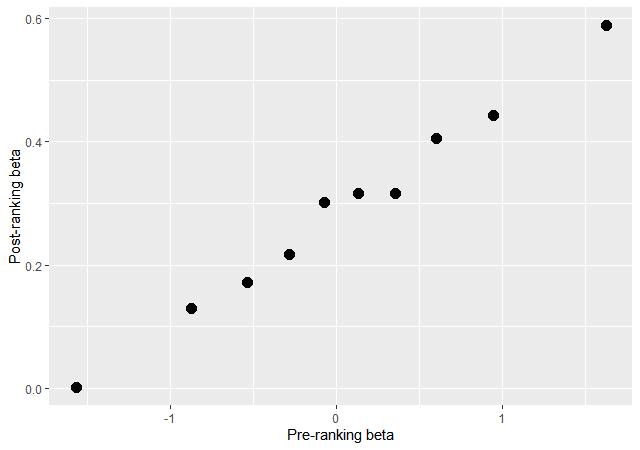
\includegraphics[width=0.94\textwidth]{paper_b3/Figure2_sl.png}
\end{frame}



\begin{frame}{Returns of decile portfolios, formed on $\beta_{CID}$}
\begin{table}[!htbp] \centering 
  \caption*{\textbf{Table 3: Returns of decile $\beta_{CID}$-sorted portfolios}}
  \label{} 
\begin{tabular}{@{\extracolsep{-6pt}} cccccccccccc} 
\\[-1.8ex]\hline 
\hline \\[-1.8ex] 
 & D1 & D2 & D3 & D4 & D5 & D6 & D7 & D8 & D9 & D10 & LS \\ 
\hline \\[-1.8ex] 
Mean ew & 2.52 & 1.78 & 1.57 & 1.42 & 1.36 & 1.32 & 1.30 & 1.26 & 1.29 & 1.61 & -0.90$^{***}$ \\ 
T-stat ew & [9.94] & [8.88] & [8.31] & [7.96] & [7.62] & [7.46] & [7.09] & [6.65] & [6.52] & [6.61] & [-5.87] \\ 
Mean vw & 1.16 & 0.88 & 0.85 & 0.73 & 0.63 & 0.66 & 0.66 & 0.61 & 0.54 & 0.49 & -0.68$^{***}$ \\ 
T-stat vw & [4.87] & [4.52] & [4.64] & [4.15] & [3.82] & [4.04] & [3.89] & [3.61] & [2.98] & [2.24] & [-3.82] \\ 
\hline \\[-1.8ex] 
\end{tabular} 
\end{table}

% Table created by stargazer v.5.2.2 by Marek Hlavac, Harvard University. E-mail: hlavac at fas.harvard.edu
% Date and time: 10/14
\begin{table}[!htbp] \centering 
  \caption*{\textbf{Table 4: Abnormal returns of decile $\beta_{CID}$-sorted vw portfolios}} 
  \label{} 
\begin{tabular}{@{\extracolsep{0pt}} ccccccc} 
\\[-1.8ex]\hline 
\hline \\[-1.8ex] 
Statistic & Ret & $\alpha_{CAPM}$ & $\alpha_{FF3}$ & $\alpha_{Carhart}$ & $\alpha_{FF5}$ & $\alpha_{FF5+UMD+STR}$ \\ 
\hline \\[-1.8ex] 
LS & -0.68$^{***}$ & -0.65$^{***}$ & -0.74$^{***}$ & -0.53$^{***}$ & -0.79$^{***}$ & -0.48$^{***}$ \\ 
T-stat & [-3.82] & [-3.63] & [-4.45] & [-3.22] & [-4.62] & [-2.85] \\ 
\hline \\[-1.8ex] 
\end{tabular} 
\end{table}
\end{frame}



\begin{frame}{Factor loadings of decile portfolios, formed on $\beta_{CID}$}
\vspace{-0.25cm}
\begin{table}[!htbp] \centering 
  \label{} 
\begin{tabular}{@{\extracolsep{0pt}} ccccccccc} 
\\[-1.8ex]\hline 
\hline \\[-1.8ex] 
Ntile & Ret & Alpha & MKT & HML & SMB & RMW & CMA & adjR2 \\ 
\hline \\[-1.8ex] 
1 & 1.16 & 0.71 & 1.03 & -0.14 & 0.44 & -0.20 & -0.30 & 0.82 \\ 
 & [ 4.87] & [ 6.70] & [ 39.08] & [ -2.70] & [ 12.05] & [ -3.99] & [ -4.01] &  \\ 
2 & 0.88 & 0.34 & 0.97 & 0.00 & 0.24 & 0.09 & -0.12 & 0.83 \\ 
 & [ 4.52] & [ 3.95] & [ 46.02] & [ 0.06] & [ 8.29] & [ 2.17] & [ -2.05] &  \\ 
3 & 0.85 & 0.36 & 0.94 & -0.05 & 0.15 & 0.01 & -0.04 & 0.83 \\ 
 & [ 4.64] & [ 4.55] & [ 47.65] & [ -1.30] & [ 5.34] & [ 0.30] & [ -0.71] &  \\ 
4 & 0.73 & 0.15 & 0.96 & 0.00 & 0.10 & 0.15 & 0.06 & 0.86 \\ 
 & [ 4.15] & [ 2.23] & [ 55.99] & [ 0.06] & [ 4.12] & [ 4.44] & [ 1.29] &  \\ 
5 & 0.63 & 0.03 & 0.93 & 0.03 & 0.09 & 0.16 & 0.18 & 0.88 \\ 
 & [ 3.82] & [ 0.42] & [ 62.47] & [ 0.99] & [ 4.12] & [ 5.58] & [ 4.22] &  \\ 
6 & 0.66 & 0.11 & 0.93 & 0.02 & 0.00 & 0.14 & 0.11 & 0.88 \\ 
 & [ 4.04] & [ 1.82] & [ 63.52] & [ 0.66] & [ 0.01] & [ 4.84] & [ 2.61] &  \\ 
7 & 0.66 & 0.09 & 0.99 & 0.05 & -0.03 & 0.10 & 0.11 & 0.90 \\ 
 & [ 3.89] & [ 1.57] & [ 70.80] & [ 2.02] & [ -1.73] & [ 3.52] & [ 2.71] &  \\ 
8 & 0.61 & -0.01 & 1.01 & 0.15 & -0.08 & 0.18 & 0.10 & 0.91 \\ 
 & [ 3.61] & [ -0.22] & [ 76.79] & [ 5.83] & [ -4.19] & [ 7.00] & [ 2.59] &  \\ 
9 & 0.54 & -0.03 & 1.03 & 0.10 & -0.11 & 0.03 & 0.06 & 0.87 \\ 
 & [ 2.98] & [ -0.37] & [ 61.80] & [ 3.20] & [ -4.58] & [ 0.88] & [ 1.17] &  \\ 
10 & 0.49 & -0.08 & 1.15 & 0.19 & -0.05 & -0.15 & -0.14 & 0.82 \\ 
 & [ 2.24] & [ -0.80] & [ 48.49] & [ 4.05] & [ -1.60] & [ -3.16] & [ -2.05] &  \\ 
LS & -0.68 & -0.79 & 0.12 & 0.32 & -0.49 & 0.06 & 0.16 & 0.16 \\ 
 & [ -3.82] & [ -4.62] & [ 2.93] & [ 3.96] & [ -8.41] & [ 0.71] & [ 1.35] &  \\ 
\hline \\[-1.8ex] 
\end{tabular} 
\end{table}
\end{frame}



{\renewcommand{\arraystretch}{0.58}
\begin{frame}{Fama-MacBeth: Table 7}
\vspace{-0.4cm}
\begin{table}[!htbp] \centering 
\begin{tabular}{@{\extracolsep{5pt}}lcccccc} 
\\[-1.8ex]\hline 
\hline \\[-1.0ex] 
 & \multicolumn{6}{c}{\textit{Dependent variable: Return}} \\ 
\cline{2-7} 
\\[-1.0ex] & (1) & (2) & (3) & (4) & (5) & (6)\\ 
\hline \\[-1.0ex] 
 $\beta_{CID}$ & $-$0.33$^{***}$ & $-$0.24$^{***}$ & $-$0.19$^{***}$ & $-$0.23$^{***}$ & $-$0.38$^{***}$ & $-$0.24$^{*}$ \\ 
  & [$-$4.37] & [$-$3.86] & [$-$2.72] & [$-$3.05] & [$-$3.69] & [$-$1.82] \\ 
  & & & & & & \\ 
 $\beta$ &  & 0.83$^{***}$ & 1.21$^{***}$ & 0.96$^{**}$ & 0.44 & 0.52 \\ 
  &  & [4.27] & [2.93] & [2.07] & [0.68] & [0.60] \\ 
  & & & & & & \\ 
 size &  &  & $-$0.06$^{*}$ & $-$0.05 & $-$0.05 & $-$0.06 \\ 
  &  &  & [$-$1.65] & [$-$1.28] & [$-$0.76] & [$-$0.80] \\ 
  & & & & & & \\ 
 logbm &  &  & 0.02 & 0.09 & 0.16 & 0.18 \\ 
  &  &  & [0.14] & [0.52] & [0.61] & [0.52] \\ 
  & & & & & & \\ 
 Momentum &  &  &  & 1.23$^{*}$ & 1.21 & 1.49 \\ 
  &  &  &  & [1.79] & [1.31] & [1.14] \\ 
  & & & & & & \\ 
 op &  &  &  &  & 2.85 & 1.79 \\ 
  &  &  &  &  & [1.49] & [0.75] \\ 
  & & & & & & \\ 
 inv &  &  &  &  & $-$0.44 & 1.28 \\ 
  &  &  &  &  & [$-$0.47] & [1.17] \\ 
  & & & & & & \\ 
 $\beta_{VOL}$ &  &  &  &  &  & 0.05 \\ 
  &  &  &  &  &  & [1.18] \\ 
  & & & & & & \\ 
 Constant & 0.68$^{***}$ & $-$0.08 & $-$0.03 & $-$0.01 & $-$0.001 & $-$0.01 \\ 
  & [4.13] & [$-$1.27] & [$-$0.61] & [$-$0.42] & [$-$0.03] & [$-$0.55] \\ 
  & & & & & & \\ 
\hline \\[-1.0ex] 
Observations & 7183 & 7183 & 7183 & 7183 & 7183 & 7183 \\ 
Adjusted R$^{2}$ & 0.44 & 0.62 & 0.77 & 0.82 & 0.90 & 0.93 \\ 
\hline 
\end{tabular} 
\end{table}
\end{frame}
}


\normalsize
\begin{frame}{CID vs WID}
\begin{itemize}
    \item {Verousis and Voukelatos (2018) find that high sensitivity to cross-sectional dispersion (CSD) predicts low returns.}
    \item {Are their results driven by across- or within-industry dispersion?}
\end{itemize}
\scriptsize
\begin{table}[!htbp] \centering 
  \caption*{\textbf{Table 8: Abnormal returns of 5x5 portfolios, double-sorted on within-industry dispersion $\beta_{WID}$ and $\beta_{CID}$}} 
  \label{} 
\begin{tabular}{@{\extracolsep{5pt}} ccccccc} 
\\[-1.8ex]\hline 
\hline \\[-1.8ex] 
Statistic & Ret & $\alpha_{CAPM}$ & $\alpha_{FF3}$ & $\alpha_{Carhart}$ & $\alpha_{FF5}$ & $\alpha_{FF5+UMD+STR}$ \\ 
\hline \\[-1.8ex] 
L/S WID & 0.16 & 0.25 & 0.13 & 0.00 & -0.12 & -0.16 \\ 
T-stat & [ 1.07] & [ 1.63] & [ 0.84] & [ 0.03] & [ -0.83] & [ -1.04] \\ 
L/S CID & 0.32$^{**}$ & 0.28$^{*}$ & 0.37$^{***}$ & 0.32$^{**}$ & 0.53$^{***}$ & 0.37$^{***}$ \\ 
T-stat & [ 2.32] & [ 1.92] & [ 2.68] & [ 2.25] & [ 3.81] & [ 2.60] \\ 
\hline \\[-1.8ex] 
\end{tabular} 
\end{table}
\end{frame}


\scriptsize
\begin{frame}{CID and volatility measures}
\begin{table}[!htbp] \centering 
  \caption*{\textbf{Table 10: Abnormal returns of 5x5 portfolios, double-sorted on $\beta_{CID}$ and other variables}}
    \begin{flushleft}
    {\medskip \scriptsize
Market volatility is a standard deviation of monthly value-weighted market returns over the last 24 months.}
    \medskip
    \end{flushleft}
\begin{tabularx}{\linewidth}{p{1.5cm}p{1cm}p{1cm}p{1cm}p{1cm}p{1cm}p{1cm}}
    \toprule
    \multicolumn{7}{l}{\textbf{Panel A: Market volatility vs CID}} \\
    \midrule 
\\[-2.5ex]\hline 
\hline \\[-1.8ex] 
Statistic & Ret & $\alpha_{CAPM}$ & $\alpha_{FF3}$ & $\alpha_{Carhart}$ & $\alpha_{FF5}$ & $\alpha_{FF5+UMD+STR}$ \\ 
\hline \\[-1.8ex] 
L/S VOL & 0.31$^{**}$ & 0.18 & 0.25$^{**}$ & 0.29$^{**}$ & 0.49$^{***}$ & 0.47$^{***}$ \\ 
T-stat & [ 2.23] & [ 1.37] & [ 1.96] & [ 2.18] & [ 3.85] & [ 3.63] \\ 
L/S CID & 0.40$^{***}$ & 0.42$^{***}$ & 0.45$^{***}$ & 0.32$^{***}$ & 0.48$^{***}$ & 0.30$^{**}$ \\ 
T-stat & [ 3.32] & [ 3.46] & [ 3.85] & [ 2.73] & [ 4.02] & [ 2.49] \\ 
\hline \\[-1.8ex] 
\end{tabularx}

\begin{tabularx}{\linewidth}{p{1.5cm}p{1cm}p{1cm}p{1cm}p{1cm}p{1cm}p{1cm}}
    \toprule
    \multicolumn{7}{l}{\textbf{Panel E: VIX vs CID}} \\
    \midrule  
\\[-2.5ex]\hline 
\hline \\[-1.8ex] 
Statistic & Ret & $\alpha_{CAPM}$ & $\alpha_{FF3}$ & $\alpha_{Carhart}$ & $\alpha_{FF5}$ & $\alpha_{FF5+UMD+STR}$ \\ 
\hline \\[-1.8ex] 
L/S VIX & 0.25 & -0.13 & -0.09 & 0.05 & 0.19 & 0.28 \\ 
T-stat & [ 1.08] & [ -0.68] & [ -0.49] & [ 0.30] & [ 1.10] & [ 1.61] \\ 
L/S CID & 0.23 & 0.23 & 0.38$^{**}$ & 0.21 & 0.30 & 0.15 \\ 
T-stat & [ 1.19] & [ 1.16] & [ 2.10] & [ 1.21] & [ 1.61] & [ 0.85] \\ 
\hline \\[-1.8ex] 
\end{tabularx} 
\end{table} 
\end{frame}



\begin{frame}{CID and uncertainty measures}
\begin{table}[!htbp] \centering 
  \caption*{\textbf{Table 10: Abnormal returns of 5x5 portfolios, double-sorted on $\beta_{CID}$ and other variables}}
  \label{} 
  \begin{flushleft}
    {\medskip
    \scriptsize
 MU and FU are macroeconomic and financial uncertainty indices from Ludvigson et al. (2015).}
    \medskip
    \end{flushleft}
\begin{tabularx}{\linewidth}{p{2cm}p{1cm}p{1cm}p{1cm}p{1cm}p{1cm}p{1cm}}
    \toprule
    \multicolumn{7}{l}{\textbf{Panel C: Macroeconomic uncertainty (Ludvigson 2015) vs CID}} \\
    \midrule  
\\[-2.5ex]\hline 
\hline \\[-1.8ex] 
Statistic & Ret & $\alpha_{CAPM}$ & $\alpha_{FF3}$ & $\alpha_{Carhart}$ & $\alpha_{FF5}$ & $\alpha_{FF5+UMD+STR}$ \\ 
\hline \\[-1.8ex] 
L/S MU & 0.05 & -0.07 & -0.03 & 0.07 & 0.19 & 0.19 \\ 
T-stat & [ 0.33] & [ -0.50] & [ -0.20] & [ 0.55] & [ 1.42] & [ 1.44] \\ 
L/S CID & 0.49$^{***}$ & 0.49$^{***}$ & 0.53$^{***}$ & 0.35$^{***}$ & 0.54$^{***}$ & 0.32$^{**}$ \\ 
T-stat & [ 3.77] & [ 3.75] & [ 4.20] & [ 2.83] & [ 4.21] & [ 2.56] \\ 
\hline \\[-1.8ex] 
\end{tabularx} 

\begin{tabularx}{\linewidth}{p{2cm}p{1cm}p{1cm}p{1cm}p{1cm}p{1cm}p{1cm}}
    \toprule
    \multicolumn{7}{l}{\textbf{Panel D: Financial uncertainty (Ludvigson 2015) vs CID}} \\
    \midrule 
\\[-2.5ex]\hline 
\hline \\[-1.8ex] 
Statistic & Ret & $\alpha_{CAPM}$ & $\alpha_{FF3}$ & $\alpha_{Carhart}$ & $\alpha_{FF5}$ & $\alpha_{FF5+UMD+STR}$ \\ 
\hline \\[-1.8ex] 
L/S FU & 0.25$^{*}$ & 0.15 & 0.01 & -0.04 & -0.10 & -0.07 \\ 
T-stat & [ 1.86] & [ 1.15] & [ 0.07] & [ -0.30] & [ -0.77] & [ -0.52] \\ 
L/S CID & 0.39$^{***}$ & 0.40$^{***}$ & 0.44$^{***}$ & 0.31$^{***}$ & 0.45$^{***}$ & 0.28$^{**}$ \\ 
T-stat & [ 3.24] & [ 3.26] & [ 3.74] & [ 2.67] & [ 3.70] & [ 2.33] \\  
\hline \\[-1.8ex] 
\end{tabularx} 
\end{table} 
\end{frame}


\normalsize
\begin{frame}{CID and CIV}
\begin{itemize}
    \item {Herskovic, Kelly, Lustig and Van Nieuwerburgh (2016) document existence of strong factor structure in idiosyncratic volatility of stock returns as well as fundamentals.}
    \item {Stocks with high exposure to common idiosyncratic volatility (CIV) earn small returns.}
    \item {They suggest a variation of the model of Constantinides and Duffie (1996) to motivate CIV as household income risk.}
    \item {How is CID different from CIV?}
\end{itemize}

\end{frame}


\footnotesize
\begin{frame}{CID and CIV: doublesorts}
\begin{table}[!htbp] \centering 
  \caption*{\textbf{Table 11: Abnormal returns of 5x5 portfolios, double-sorted on $\beta_{CID}$ and $\beta_{CIV}$}}
  \label{} 
  \begin{flushleft}
    {\medskip \scriptsize
 The table reports abnormal monthly returns of long-short value-weighted portfolios, formed from independent 5 by 5 double sorts on $\beta_{CID}$ and $\beta_{CIV}$. CIV is common idiosyncratic volatility from Herskovic, Kelly, Lustig and Van Nieuwerburgh (2016). }
    \medskip
    \end{flushleft}
\begin{tabular}{@{\extracolsep{5pt}} ccccccc} 
\\[-1.8ex]\hline 
\hline \\[-1.8ex] 
Statistic & Ret & $\alpha_{CAPM}$ & $\alpha_{FF3}$ & $\alpha_{Carhart}$ & $\alpha_{FF5}$ & $\alpha_{FF5+UMD+STR}$ \\ 
\hline \\[-1.8ex] 
L/S CIV & 0.33$^{***}$ & 0.27$^{**}$ & 0.17 & 0.21$^{*}$ & 0.08 & 0.13 \\ 
T-stat & [ 2.78] & [ 2.28] & [ 1.43] & [ 1.78] & [ 0.68] & [ 1.07] \\ 
L/S CID & 0.37$^{***}$ & 0.39$^{***}$ & 0.42$^{***}$ & 0.26$^{**}$ & 0.44$^{***}$ & 0.23$^{**}$ \\ 
T-stat & [ 3.06] & [ 3.22] & [ 3.64] & [ 2.27] & [ 3.71] & [ 1.99] \\ 
\hline \\[-1.8ex] 
\end{tabular} 
\end{table}
\end{frame}



\scriptsize
{\renewcommand{\arraystretch}{0.56}
\begin{frame}{CID and CIV: Spanning tests between the two factors}
\vspace{-0.3cm}
\begin{table}[!htbp] \centering 
\begin{tabular}{@{\extracolsep{5pt}}lcccc} 
\\[-1ex]\hline 
\hline \\[-1.8ex] 
 & \multicolumn{4}{c}{\textit{Dependent variable:}} \\ 
\cline{2-5} 
\\[-1ex] & \multicolumn{2}{c}{CID factor} & \multicolumn{2}{c}{CIV factor} \\ 
\\[-1.8ex] & (1) & (2) & (3) & (4)\\ 
\hline \\[-1ex] 
 MKT & 0.110$^{**}$ & 0.151$^{***}$ & $-$0.117$^{***}$ & $-$0.154$^{***}$ \\ 
  & [2.562] & [3.710] & [$-$2.727] & [$-$3.827] \\ 
  & & & & \\ 
 SMB & $-$0.500$^{***}$ & $-$0.376$^{***}$ & $-$0.359$^{***}$ & $-$0.187$^{***}$ \\ 
  & [$-$8.192] & [$-$6.364] & [$-$5.909] & [$-$3.105] \\ 
  & & & & \\ 
 HML & 0.156$^{*}$ & 0.138$^{*}$ & 0.054 & 0.0004 \\ 
  & [1.813] & [1.697] & [0.631] & [0.004] \\ 
  & & & & \\ 
 RMW & 0.080 & 0.177$^{**}$ & $-$0.277$^{***}$ & $-$0.305$^{***}$ \\ 
  & [0.951] & [2.215] & [$-$3.319] & [$-$3.882] \\ 
  & & & & \\ 
 CMA & 0.401$^{***}$ & 0.399$^{***}$ & 0.006 & $-$0.131 \\ 
  & [3.144] & [3.329] & [0.051] & [$-$1.095] \\ 
  & & & & \\ 
 Mom & $-$0.274$^{***}$ & $-$0.284$^{***}$ & 0.029 & 0.123$^{***}$ \\ 
  & [$-$6.610] & [$-$7.300] & [0.716] & [3.087] \\ 
  & & & & \\ 
 CIV factor &  & 0.348$^{***}$ &  &  \\ 
  &  & [9.009] &  &  \\ 
  & & & & \\ 
 CID factor &  &  &  & 0.344$^{***}$ \\ 
  &  &  &  & [9.009] \\ 
  & & & & \\ 
 Constant & $-$0.652$^{***}$ & $-$0.503$^{***}$ & $-$0.427$^{**}$ & $-$0.203 \\ 
  & [$-$3.656] & [$-$2.991] & [$-$2.411] & [$-$1.207] \\ 
  & & & & \\ 
\hline \\[-1ex] 
Observations & 605 & 605 & 605 & 605 \\ 
Adjusted R$^{2}$ & 0.222 & 0.314 & 0.078 & 0.187 \\ 
\hline 
\hline \\[-1.8ex] 
\end{tabular} 
\end{table}
\end{frame}
}
\footnotesize


\begin{frame}{Other industry classifications}
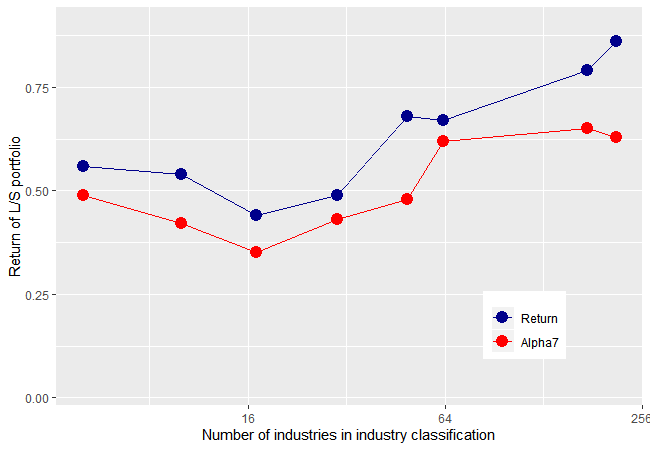
\includegraphics[width=0.94\textwidth]{paper_b3/Figure4_sl.png}
\end{frame}



\begin{frame}{CID vs WID using FF5 industry classification}
\begin{table}[!htbp] \centering 
  \caption*{\textbf{Table 16: Abnormal returns of 5x5 portfolios, double-sorted on within-industry dispersion $\beta_{WID}$ and $\beta_{CID}$} using FF5 industry classification} 
  \label{} 
  \begin{flushleft}
    {\medskip\scriptsize
 The table reports abnormal monthly returns of long-short value-weighted portfolios, formed from independent 5 by 5 double sorts on $\beta_{WID}$ and $\beta_{CID}$. WID (within-industry dispersion) is a mean absolute deviation of returns of the stocks within each industry, averaged across 5 industries.}
    \medskip
    \end{flushleft}
\begin{tabular}{@{\extracolsep{5pt}} ccccccc} 
\\[-1.8ex]\hline 
\hline \\[-1.8ex] 
Statistic & Ret & $\alpha_{CAPM}$ & $\alpha_{FF3}$ & $\alpha_{Carhart}$ & $\alpha_{FF5}$ & $\alpha_{FF5+UMD+STR}$ \\ 
\hline \\[-1.8ex] 
L/S WID & 0.22^{*} & 0.30^{***} & 0.24^{**} & 0.13 & 0.06 & -0.03 \\ 
T-stat & [ 1.92] & [ 2.69] & [ 2.16] & [ 1.18] & [ 0.56] & [ -0.31] \\ 
L/S CID & 0.20 & 0.18 & 0.27^{**} & 0.21 & 0.39^{***} & 0.21 \\ 
T-stat & [ 1.48] & [ 1.38] & [ 2.10] & [ 1.57] & [ 2.97] & [ 1.61] \\ 
\hline \\[-1.8ex] 
\end{tabular} 
\end{table}
\end{frame}


\normalsize
\begin{frame}{Economic channel: labor risk}
\begin{itemize}
    \item {Accelerated rate of sectoral reallocation of resources brings unemployment risk for employees in declining industries.}
    \item {This risk has larger magnitude and longer-lasting consequences for workers with industry-specific skills.}
    \item {Losing the job in declining industry constitutes large negative shock to expected lifetime labor income.}
    \item {An increase in CID reflects an increase in labor income risk.}
    \item {Given incomplete insurance of labor risk, it should matter for asset pricing.}
\end{itemize}
\end{frame}



\begin{frame}{Sectoral shifts hypothesis}
\begin{itemize}
    \item {Lilien(1982): Unemployment is driven by two types of shocks:}
    \begin{itemize}
        \item {Aggregate shocks.}
        \item {Reallocation shocks.}
    \end{itemize}
    \item {Aggregate shocks represent short-term fluctuations in business activity, while reallocation shocks reflect persistent changes in sectoral composition of the economy.}
    \item {While aggregate shocks have transitory effect on unemployment, reallocation shocks are more long-term in nature.}
    \item {Lilien (1982), Loungani et al.(1990) and Brainard et al.(1993) document that the variance in employment growth and returns across industries predict aggregate unemploymnet growth at the annual frequency.}
\end{itemize}
\end{frame}


\scriptsize
{\renewcommand{\arraystretch}{0.8}
\begin{frame}{Unemployment predictability}
\begin{table}[!htbp] \centering 
  \caption*{\textbf{Table 15: Predictive regressions for unemployment}} 
\begin{tabular}{@{\extracolsep{-2pt}}lcccccc} 
\\[-1.8ex]\hline 
\hline \\[-1.5ex] 
 & \multicolumn{6}{c}{\textit{Dependent variable:}} \\ 
\cline{2-7} \\[-1ex]
 & \multicolumn{2}{c}{Unemployment growth} & \multicolumn{2}{c}{LT Unemployment growth} & \multicolumn{2}{c}{ST Unemployment growth} \\ 
\\[-1.8ex] & (1) & (2) & (3) & (4) & (5) & (6)\\ 
\hline \\[-1ex] 
 $CID_{t-1}$ & 3.70$^{***}$ & 3.30$^{**}$ & 2.29$^{**}$ & 1.95$^{**}$ & 0.25 & 0.22 \\ 
  & [2.72] & [2.53] & [2.03] & [2.04] & [0.57] & [0.54] \\ 
  & & & & & & \\ 
 $Mkt_{t-1}$ &  & $-$0.88$^{***}$ &  & $-$0.03 &  & $-$0.41$^{***}$ \\ 
  &  & [$-$2.96] &  & [$-$0.17] &  & [$-$4.38] \\ 
  & & & & & & \\ 
 $Vol_{t-1}$ &  & 0.20$^{**}$ &  & 0.10$^{**}$ &  & 0.05$^{**}$ \\ 
  &  & [2.45] &  & [2.15] &  & [1.96] \\ 
  & & & & & & \\ 
 Constant & $-$0.0002 & $-$0.0004 & 0.003 & 0.003 & $-$0.003 & $-$0.003 \\ 
  & [$-$0.004] & [$-$0.01] & [0.09] & [0.11] & [$-$0.35] & [$-$0.40] \\ 
  & & & & & & \\ 
\hline \\[-1.8ex] 
Observations & 284 & 284 & 284 & 284 & 284 & 284 \\ 
R$^{2}$ & 0.03 & 0.11 & 0.03 & 0.06 & 0.001 & 0.11 \\ 
Adjusted R$^{2}$ & 0.02 & 0.10 & 0.03 & 0.05 & $-$0.002 & 0.10 \\ 
\hline 
\hline \\[-1.8ex] 
\end{tabular} 
\end{table}
\end{frame}
}



\normalsize
\begin{frame}{Future work}
\begin{itemize}
    \item {I plan to perform cross-sectional tests of employment predictability}
    \begin{itemize}
        \item {Do returns of industry portfolios predict employment?}
        \item {Does high CID predict low employment growth in outperforming or underperforming industries?}
    \end{itemize}
    \item {So far I used product market-based industry classifications.}
    \item {I plan to use occupation-driven industry classifications to construct CID.}
\end{itemize}
\end{frame}


\normalsize
\begin{frame}{Conclusion}
\begin{itemize}
    \item {Stocks with high sensitivity to CID produce low returns.}
    \item {The long-short strategy, based on $\beta_{CID}$, delivers 48-79 bps of monthly abnormal returns.}
    \item {Unlike cross-industry dispersion, within-industry dispersion is not priced.}
    \item {CID subsumes a large fraction of CIV premium.}
    \item {High innovations in CID predict high unemployment growth.}
    \item {Results are consistent with CID proxying for unemployment risk from sectoral shifts.}
\end{itemize}
\end{frame}



\footnotesize
{\renewcommand{\arraystretch}{0.72}
\begin{frame}{Appendix: $\beta_{CID}$ of FF49 industries}
% Table created by stargazer v.5.2.2 by Marek Hlavac, Harvard University. E-mail: hlavac at fas.harvard.edu
% Date and time: Wed, Oct 30, 2019 - 2:15:25 PM
\begin{table}[!htbp] \centering 
\begin{tabular}{@{\extracolsep{5pt}} cccc} 
\\[-1.8ex]\hline 
\hline \\[-1.8ex] 
Industry & $\beta_{CID}$ & Industry & $\beta_{CID}$ \\ 
\hline \\[-1.8ex] 
Boxes & $$-$1.52$ & Fun & $$-$0.22$ \\ 
Coal & $$-$1.25$ & Rubbr & $$-$0.21$ \\ 
Ships & $$-$1.24$ & Chems & $$-$0.20$ \\ 
Txtls & $$-$0.83$ & Chips & $$-$0.20$ \\ 
PerSv & $$-$0.81$ & Hshld & $$-$0.19$ \\ 
Mines & $$-$0.68$ & BldMt & $$-$0.18$ \\ 
FabPr & $$-$0.55$ & Util & $$-$0.18$ \\ 
Aero & $$-$0.54$ & Steel & $$-$0.18$ \\ 
Agric & $$-$0.53$ & Beer & $$-$0.16$ \\ 
Hlth & $$-$0.51$ & Cnstr & $$-$0.16$ \\ 
Toys & $$-$0.46$ & MedEq & $$-$0.16$ \\ 
Insur & $$-$0.46$ & LabEq & $$-$0.14$ \\ 
Whlsl & $$-$0.46$ & Telcm & $$-$0.12$ \\ 
Meals & $$-$0.45$ & Paper & $$-$0.07$ \\ 
Fin & $$-$0.44$ & RlEst & $$-$0.04$ \\ 
BusSv & $$-$0.43$ & Drugs & $$-$0.03$ \\ 
Mach & $$-$0.42$ & Autos & $0.08$ \\ 
Oil & $$-$0.38$ & Other & $0.11$ \\ 
Trans & $$-$0.35$ & Books & $0.14$ \\ 
Rtail & $$-$0.34$ & Hardw & $0.14$ \\ 
Clths & $$-$0.27$ & Softw & $0.23$ \\ 
Banks & $$-$0.26$ & Soda & $1.02$ \\ 
Food & $$-$0.26$ & Guns & $1.30$ \\ 
ElcEq & $$-$0.26$ & Gold & $1.58$ \\ 
\hline \\[-1.8ex] 
\end{tabular} 
\end{table}
\end{frame}
}



\scriptsize
{\renewcommand{\arraystretch}{0.72}
\begin{frame}{Appendix: Fama-MacBeth across stocks}
\vspace{-0.3cm}
\begin{table}[!htbp] \centering 
\begin{tabular}{@{\extracolsep{-4pt}}lccccccc} 
\\[-1.8ex]\hline 
\hline \\[-1.8ex] 
 & \multicolumn{7}{c}{\textit{Dependent variable: Return}} \\ 
\cline{2-8} 
\\[-1.8ex] & (1) & (2) & (3) & (4) & (5) & (6) & (7)\\ 
\hline \\[-1.8ex] 
 beta\_cid & $-$0.31$^{***}$ & $-$0.31$^{***}$ & $-$0.10$^{**}$ & $-$0.09$^{**}$ & $-$0.08$^{**}$ & $-$0.09$^{**}$ & $-$0.09$^{**}$ \\ 
  & [$-$5.35] & [$-$6.81] & [$-$2.51] & [$-$2.50] & [$-$2.34] & [$-$2.41] & [$-$2.40] \\ 
  & & & & & & & \\ 
 beta &  & 0.38 & 1.18$^{***}$ & 1.18$^{***}$ & 1.04$^{***}$ & 1.19$^{***}$ & 0.95$^{***}$ \\ 
  &  & [1.29] & [3.60] & [3.81] & [3.52] & [3.98] & [3.38] \\ 
  & & & & & & & \\ 
 size &  &  & $-$0.64$^{***}$ & $-$0.64$^{***}$ & $-$0.63$^{***}$ & $-$0.64$^{***}$ & $-$0.59$^{***}$ \\ 
  &  &  & [$-$14.88] & [$-$14.24] & [$-$14.61] & [$-$14.88] & [$-$15.22] \\ 
  & & & & & & & \\ 
 logbm &  &  &  & 0.01 & 0.02 & $-$0.05 & $-$0.02 \\ 
  &  &  &  & [0.20] & [0.34] & [$-$0.90] & [$-$0.40] \\ 
  & & & & & & & \\ 
 mom122 &  &  &  &  & 0.22 & 0.12 & 0.15 \\ 
  &  &  &  &  & [1.13] & [0.65] & [0.79] \\ 
  & & & & & & & \\ 
 inv &  &  &  &  &  & $-$1.25$^{***}$ & $-$1.26$^{***}$ \\ 
  &  &  &  &  &  & [$-$8.47] & [$-$8.60] \\ 
  & & & & & & & \\ 
 MAX &  &  &  &  &  &  & 0.04$^{***}$ \\ 
  &  &  &  &  &  &  & [5.54] \\ 
  & & & & & & & \\ 
 Constant & 1.48$^{***}$ & 1.13$^{***}$ & 4.14$^{***}$ & 4.19$^{***}$ & 4.24$^{***}$ & 3.84$^{***}$ & 3.69$^{***}$ \\ 
  & [8.19] & [6.98] & [17.30] & [10.25] & [10.38] & [9.38] & [8.94] \\ 
  & & & & & & & \\ 
\hline \\[-1.8ex] 
Observations & 1,726,983 & 1,726,983 & 1,262,126 & 1,262,126 & 1,259,604 & 1,230,210 & 1,230,207 \\ 
Adjusted R$^{2}$ & 0.01 & 0.04 & 0.05 & 0.06 & 0.07 & 0.07 & 0.07 \\ 
\hline 
\hline \\[-1.8ex] 
\end{tabular} 
\end{table}
\end{frame}
}



\scriptsize
\begin{frame}{Appendix: CID, constructed from abnormal industry returns}
% the following two tables were updated on 10/21 using SP19_rm_35 script with betas from "crsp_dailyindmadbetas504_2_ff5_v1.csv".
% Table created by stargazer v.5.2.2 by Marek Hlavac, Harvard University. E-mail: hlavac at fas.harvard.edu
% Date and time: Sat, Sep 14, 2019 - 4:33:56 PM
\begin{table}[!htbp] \centering 
  \caption{\textbf{Returns of the decile portfolios, formed on $\beta_{CID}$, calculated from abnormal returns of FF49 industry portfolios}} 
  \label{} 
  \vspace{-0.4cm}
\begin{tabular}{@{\extracolsep{-11pt}} cccccccccccc} 
\\[-1.8ex]\hline 
\hline \\[-1.8ex] 
 & D1 & D2 & D3 & D4 & D5 & D6 & D7 & D8 & D9 & D10 & LS \\ 
\hline \\[-1.8ex] 
Mean ew & 2.53^{***} & 1.82^{***} & 1.53^{***} & 1.41^{***} & 1.33^{***} & 1.30^{***} & 1.28^{***} & 1.29^{***} & 1.38^{***} & 1.75^{***} & -0.77^{***} \\ 
T-stat ew & [9.98] & [9.04] & [8.11] & [7.71] & [7.31] & [7.05] & [6.80] & [6.51] & [6.54] & [6.72] & [-5.17] \\ 
Mean vw & 1.21^{***} & 0.93^{***} & 0.79^{***} & 0.70^{***} & 0.64^{***} & 0.53^{***} & 0.62^{***} & 0.59^{***} & 0.53^{***} & 0.55^{**} & -0.66^{***} \\ 
T-stat vw & [5.04] & [4.69] & [4.31] & [3.98] & [3.73] & [3.15] & [3.62] & [3.29] & [2.78] & [2.38] & [-3.64] \\ 
\hline \\[-1.8ex] 
\end{tabular} 
\end{table}



% Table created by stargazer v.5.2.2 by Marek Hlavac, Harvard University. E-mail: hlavac at fas.harvard.edu
% Date and time: Sat, Sep 14, 2019 - 4:34:17 PM
\begin{table}[!htbp] \centering 
  \caption{\textbf{Abnormal returns of the long-short portfolio, formed on $\beta_{CID}$, calculated from abnormal returns of FF49 industry portfolios}} 
  \label{} 
  \vspace{-0.4cm}
\begin{tabular}{@{\extracolsep{5pt}} ccccccc} 
\\[-1.8ex]\hline 
\hline \\[-1.8ex] 
Statistic & Ret & $\alpha_{CAPM}$ & $\alpha_{FF3}$ & $\alpha_{Carhart}$ & $\alpha_{FF5}$ & $\alpha_{FF5+UMD+STR}$ \\ 
\hline \\[-1.8ex] 
LS Return & -0.66^{***} & -0.65^{***} & -0.77^{***} & -0.58^{***} & -0.85^{***} & -0.60^{***} \\ 
T-stat & [-3.64] & [-3.58] & [-4.46] & [-3.35] & [-4.78] & [-3.38] \\  
\hline \\[-1.8ex] 
\end{tabular} 
\end{table}
\end{frame}



{\renewcommand{\arraystretch}{0.50}
\begin{frame}{Appendix: CID vs CID: Fama-MacBeth across $\beta_{CID}$-sorted portfolios}
\vspace{-0.4cm}
\begin{table}[!htbp] \centering 
\begin{tabular}{@{\extracolsep{-2pt}}lccccccc} 
\\[-1.8ex]\hline 
\hline \\[-1.8ex] 
 & \multicolumn{7}{c}{\textit{Dependent variable: Return}} \\ 
\cline{2-8} 
\\[-1.8ex] & (1) & (2) & (3) & (4) & (5) & (6) & (7)\\ 
\hline \\[-1.0ex] 
 $\beta_{CID}$ & $-$0.33$^{***}$ & $-$0.24$^{***}$ & $-$0.19$^{***}$ & $-$0.23$^{***}$ & $-$0.38$^{***}$ & $-$0.24$^{*}$ & $-$0.09 \\ 
  & [$-$4.37] & [$-$3.86] & [$-$2.72] & [$-$3.05] & [$-$3.69] & [$-$1.82] & [$-$0.27] \\ 
  & & & & & & & \\ 
 $\beta$ &  & 0.83$^{***}$ & 1.21$^{***}$ & 0.96$^{**}$ & 0.44 & 0.52 & $-$2.73 \\ 
  &  & [4.27] & [2.93] & [2.07] & [0.68] & [0.60] & [$-$1.02] \\ 
  & & & & & & & \\ 
 size &  &  & $-$0.06$^{*}$ & $-$0.05 & $-$0.05 & $-$0.06 & 0.22 \\ 
  &  &  & [$-$1.65] & [$-$1.28] & [$-$0.76] & [$-$0.80] & [0.99] \\ 
  & & & & & & & \\ 
 logbm &  &  & 0.02 & 0.09 & 0.16 & 0.18 & $-$0.11 \\ 
  &  &  & [0.14] & [0.52] & [0.61] & [0.52] & [$-$0.13] \\ 
  & & & & & & & \\ 
 Momentum &  &  &  & 1.23$^{*}$ & 1.21 & 1.49 & $-$2.74 \\ 
  &  &  &  & [1.79] & [1.31] & [1.14] & [$-$0.80] \\ 
  & & & & & & & \\ 
 op &  &  &  &  & 2.85 & 1.79 & 4.18 \\ 
  &  &  &  &  & [1.49] & [0.75] & [0.72] \\ 
  & & & & & & & \\ 
 inv &  &  &  &  & $-$0.44 & 1.28 & 2.63 \\ 
  &  &  &  &  & [$-$0.47] & [1.17] & [1.13] \\ 
  & & & & & & & \\ 
 $\beta_{VOL}$ &  &  &  &  &  & 0.05 & $-$0.003 \\ 
  &  &  &  &  &  & [1.18] & [$-$0.03] \\ 
  & & & & & & & \\ 
 $\beta_{CIV}$ &  &  &  &  &  &  & 0.11 \\ 
  &  &  &  &  &  &  & [0.78] \\ 
  & & & & & & & \\ 
 Constant & 0.68$^{***}$ & $-$0.08 & $-$0.03 & $-$0.01 & $-$0.001 & $-$0.01 & $-$0.03$^{**}$ \\ 
  & [4.13] & [$-$1.27] & [$-$0.61] & [$-$0.42] & [$-$0.03] & [$-$0.55] & [$-$2.11] \\ 
  & & & & & & & \\ 
\hline \\[-1.8ex] 
Observations & 7183 & 7183 & 7183 & 7183 & 7183 & 7183 & 7183 \\ 
Adjusted R$^{2}$ & 0.44 & 0.62 & 0.77 & 0.82 & 0.90 & 0.93 & 0.97 \\ 
\hline 
\hline \\[-1.8ex] 
\textit{Note:}  & \multicolumn{7}{r}{$^{*}$p$<$0.1; $^{**}$p$<$0.05; $^{***}$p$<$0.01} \\ 
\end{tabular} 
\end{table}
\end{frame}
}



{\renewcommand{\arraystretch}{0.50}
\begin{frame}{Appendix: CID vs CIV: Fama-MacBeth across $\beta_{CIV}$-sorted portfolios}
\vspace{-0.4cm}
\begin{table}[!htbp] \centering 
\begin{tabular}{@{\extracolsep{-2pt}}lccccccc} 
\\[-1.8ex]\hline 
\hline \\[-1.8ex] 
 & \multicolumn{7}{c}{\textit{Dependent variable: Return}} \\ 
\cline{2-8} 
\\[-1.8ex] & (1) & (2) & (3) & (4) & (5) & (6) & (7)\\ 
\hline \\[-1.0ex] 
 $\beta_{CIV}$ & $-$0.05$^{***}$ & $-$0.03$^{***}$ & $-$0.04$^{***}$ & $-$0.04$^{***}$ & $-$0.04$^{**}$ & $-$0.06 & $-$0.07 \\ 
  & [$-$4.30] & [$-$2.98] & [$-$3.36] & [$-$3.12] & [$-$2.10] & [$-$1.45] & [$-$1.07] \\ 
  & & & & & & & \\ 
 $\beta$ &  & 0.55$^{***}$ & 0.61 & 0.12 & 0.59 & 1.61$^{**}$ & 5.41$^{**}$ \\ 
  &  & [2.81] & [1.36] & [0.25] & [0.91] & [1.98] & [2.50] \\ 
  & & & & & & & \\ 
 size &  &  & $-$0.01 & 0.01 & $-$0.06 & $-$0.13$^{*}$ & $-$0.44$^{***}$ \\ 
  &  &  & [$-$0.25] & [0.25] & [$-$0.91] & [$-$1.72] & [$-$3.02] \\ 
  & & & & & & & \\ 
 logbm &  &  & 0.17 & 0.30$^{*}$ & 0.18 & 0.26 & 0.73 \\ 
  &  &  & [1.08] & [1.83] & [0.80] & [0.91] & [1.31] \\ 
  & & & & & & & \\ 
 Momentum &  &  &  & 0.97 & 0.45 & $-$0.61 & $-$1.47 \\ 
  &  &  &  & [1.43] & [0.52] & [$-$0.55] & [$-$0.56] \\ 
  & & & & & & & \\ 
 op &  &  &  &  & 1.01 & 1.30 & 9.97$^{**}$ \\ 
  &  &  &  &  & [0.54] & [0.54] & [2.36] \\ 
  & & & & & & & \\ 
 inv &  &  &  &  & 0.11 & $-$0.26 & $-$6.56 \\ 
  &  &  &  &  & [0.09] & [$-$0.17] & [$-$0.95] \\ 
  & & & & & & & \\ 
 $\beta_{VOL}$ &  &  &  &  &  & $-$0.06 & $-$0.04 \\ 
  &  &  &  &  &  & [$-$1.16] & [$-$0.46] \\ 
  & & & & & & & \\ 
 $\beta_{CID}$ &  &  &  &  &  &  & $-$0.49 \\ 
  &  &  &  &  &  &  & [$-$0.49] \\ 
  & & & & & & & \\ 
 Constant & 0.48$^{***}$ & 0.005 & 0.03 & 0.07$^{*}$ & 0.04 & 0.01 & $-$0.01 \\ 
  & [3.03] & [0.08] & [0.73] & [1.88] & [1.25] & [0.33] & [$-$0.85] \\ 
  & & & & & & & \\ 
\hline \\[-1.8ex] 
Observations & 7183 & 7183 & 7183 & 7183 & 7183 & 7183 & 7183 \\ 
Adjusted R$^{2}$ & 0.46 & 0.59 & 0.73 & 0.79 & 0.88 & 0.92 & 0.96 \\ 
\hline 
\hline \\[-1.8ex] 
\textit{Note:}  & \multicolumn{7}{r}{$^{*}$p$<$0.1; $^{**}$p$<$0.05; $^{***}$p$<$0.01} \\ 
\end{tabular} 
\end{table}
\end{frame}
}



\begin{frame}{Appendix: 2x3 Doublesort on $\beta_{CID}$ and size}
\begin{table}[!htbp] \centering 
  \caption{\textbf{Abnormal returns of 2x3 doublesorted portfolios on size and $\beta_{CID}$}}
  \label{} 
\begin{tabular}{@{\extracolsep{5pt}} ccccccc} 
\\[-1.8ex]\hline 
\hline \\[-1.8ex] 
Statistic & Ret & $\alpha_{CAPM}$ & $\alpha_{FF3}$ & $\alpha_{Carhart}$ & $\alpha_{FF5}$ & $\alpha_{FF5+UMD+STR}$ \\ 
\hline \\[-1.8ex] 
L/S Size & 0.73$^{***}$ & 0.66$^{***}$ & 0.50$^{***}$ & 0.56$^{***}$ & 0.47$^{***}$ & 0.52$^{***}$ \\ 
T-stat & [ 7.42] & [ 6.84] & [ 12.48] & [ 14.00] & [ 11.44] & [ 12.77] \\ 
L/S CID & 0.21$^{**}$ & 0.23$^{**}$ & 0.28$^{***}$ & 0.15 & 0.31$^{***}$ & 0.15 \\ 
T-stat & [ 2.21] & [ 2.39] & [ 2.97] & [ 1.62] & [ 3.19] & [ 1.62] \\ 
\hline \\[-1.8ex] 
\end{tabular} 
\end{table}
\end{frame}



{\renewcommand{\arraystretch}{0.95}
\begin{frame}{Appendix: FF7 Factor loadings}
\vspace{-0.5cm}
\begin{table}[!htbp] \centering 
\begin{tabular}{@{\extracolsep{-5pt}} ccccccccccc} 
\\[-1.8ex]\hline 
\hline \\[-1.8ex] 
Decile & Ret & Alpha & EMKT & HML & SMB & RMW & CMA & Mom & STR & R2 \\ 
\hline \\[-1.8ex] 
1 & 1.16 & 0.54 & 1.03 & -0.08 & 0.42 & -0.24 & -0.33 & 0.16 & 0.13 & 0.83 \\ 
 & [ 4.87] & [ 5.15] & [ 39.22] & [ -1.50] & [ 11.80] & [ -4.79] & [ -4.55] & [ 6.44] & [ 3.64] &  \\ 
2 & 0.88 & 0.21 & 0.97 & 0.05 & 0.23 & 0.06 & -0.15 & 0.12 & 0.10 & 0.84 \\ 
 & [ 4.52] & [ 2.50] & [ 45.91] & [ 1.13] & [ 7.94] & [ 1.58] & [ -2.47] & [ 5.86] & [ 3.47] &  \\ 
3 & 0.85 & 0.26 & 0.95 & 0.01 & 0.14 & -0.02 & -0.08 & 0.12 & 0.04 & 0.84 \\ 
 & [ 4.64] & [ 3.25] & [ 48.19] & [ 0.18] & [ 5.05] & [ -0.45] & [ -1.37] & [ 6.49] & [ 1.53] &  \\ 
4 & 0.73 & 0.07 & 0.96 & 0.03 & 0.09 & 0.13 & 0.05 & 0.08 & 0.07 & 0.86 \\ 
 & [ 4.15] & [ 1.02] & [ 55.37] & [ 0.93] & [ 3.73] & [ 3.97] & [ 0.99] & [ 4.80] & [ 2.90] &  \\ 
5 & 0.63 & -0.02 & 0.94 & 0.05 & 0.08 & 0.15 & 0.17 & 0.04 & 0.02 & 0.88 \\ 
 & [ 3.82] & [ -0.25] & [ 61.21] & [ 1.61] & [ 3.90] & [ 5.23] & [ 3.93] & [ 3.02] & [ 1.08] &  \\ 
6 & 0.66 & 0.07 & 0.93 & 0.02 & -0.01 & 0.13 & 0.11 & 0.02 & 0.06 & 0.88 \\ 
 & [ 4.04] & [ 1.14] & [ 61.66] & [ 0.71] & [ -0.29] & [ 4.70] & [ 2.67] & [ 1.65] & [ 2.84] &  \\ 
7 & 0.66 & 0.09 & 0.98 & 0.03 & -0.04 & 0.10 & 0.13 & -0.02 & 0.05 & 0.90 \\ 
 & [ 3.89] & [ 1.48] & [ 68.60] & [ 1.21] & [ -1.87] & [ 3.80] & [ 3.17] & [ -1.66] & [ 2.75] &  \\ 
8 & 0.61 & 0.02 & 1.01 & 0.13 & -0.07 & 0.19 & 0.11 & -0.04 & 0.00 & 0.91 \\ 
 & [ 3.61] & [ 0.31] & [ 74.74] & [ 4.95] & [ -4.03] & [ 7.33] & [ 2.91] & [ -2.89] & [ -0.24] &  \\ 
9 & 0.54 & 0.05 & 1.03 & 0.06 & -0.10 & 0.05 & 0.08 & -0.09 & -0.03 & 0.88 \\ 
 & [ 2.98] & [ 0.71] & [ 60.90] & [ 1.97] & [ -4.30] & [ 1.51] & [ 1.70] & [ -5.27] & [ -1.34] &  \\ 
10 & 0.49 & 0.07 & 1.16 & 0.14 & -0.03 & -0.12 & -0.12 & -0.13 & -0.13 & 0.83 \\ 
 & [ 2.24] & [ 0.69] & [ 48.68] & [ 3.04] & [ -1.06] & [ -2.62] & [ -1.76] & [ -5.74] & [ -3.98] &  \\ 
LS & -0.68 & -0.48 & 0.13 & 0.22 & -0.46 & 0.12 & 0.22 & -0.30 & -0.25 & 0.23 \\ 
 & [ -3.82] & [ -2.85] & [ 3.11] & [ 2.68] & [ -8.05] & [ 1.52] & [ 1.86] & [ -7.34] & [ -4.57] &  \\ 
\hline \\[-1.8ex] 
\end{tabular} 
\end{table} 
\end{frame}
}



\end{document}

